\documentclass{article}
\usepackage[margin=1.25in]{geometry}
\usepackage{amsmath, amssymb, setspace, enumerate, enumitem}
\usepackage{setspace}
\usepackage{graphicx}
\onehalfspacing

\begin{document}
    \begin{enumerate}
        \item Exercise 1.8 in LFD
        \begin{center}
            binomial distribution tells us
        \end{center}
        \begin{align*}
            p_x &= {n \choose x} p^x q^{n-x}\\
            n &= 10\\
            x &= 0 \text{ and } x = 1\\
            p &= 0.9\\
            q &= 1 - p = 0.1\\
            p_0 &= {10 \choose 0} 0.9^0 0.1^{10} = 0.1^{10} = 1 \times 10^{-10}\\
            p_1 &= {10 \choose 1} 0.9^1 0.1^9 = 10 \times 0.9 \times 0.1^9 = 9 \times 10^{-9}\\
            p&= p_0 + p_1 = 9.1 \times 10^{-9}
        \end{align*}

        \item Exercise 1.9 in LFD\\[0.25in]
        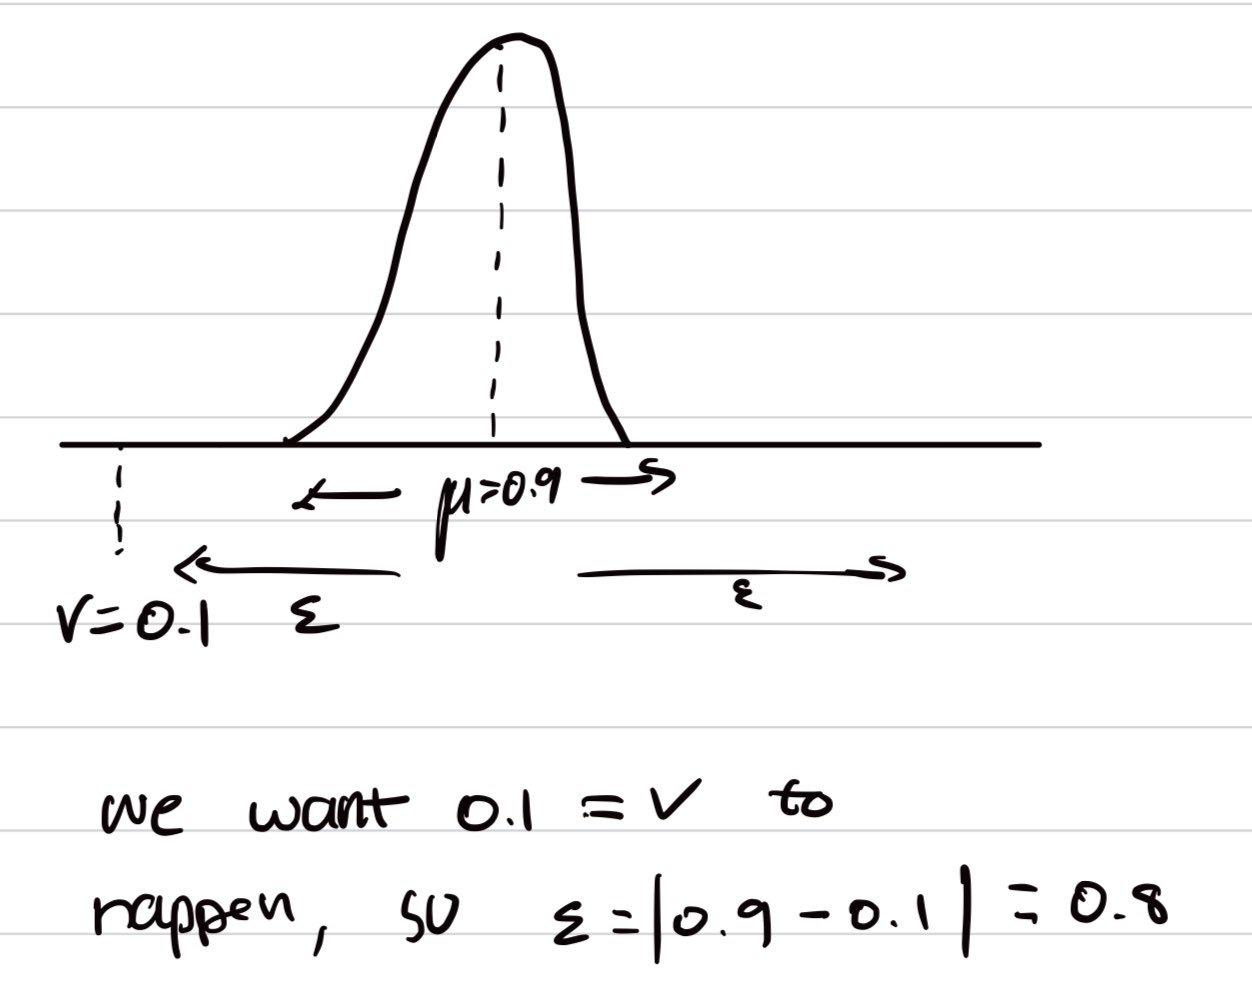
\includegraphics[scale=0.2]{images/1.9.jpg}\\[0.25in]
        Using $P[ |\nu - \mu| \geq \epsilon] \leq 2e^{-2\epsilon^2N}$, we can find the following bounds:\\
        Using $\epsilon = 0.8$ and $N = 10$, we can derive $2e^{-2\epsilon^2N} = 2e^{2(0.8)^2 \times 10}$, which equals $5.52 \times 10^{-6}$.\\
        Since this is a bound, it is reasonable for it to be greater than our answer in exercise 1.8

        \item Exercise 1.10 in LFD
        \begin{enumerate}[label=(\alph*)]
            \item $\mu = 0.5$
            \item \textbf{FINISH HERE}
            \item \textbf{FINISH HERE}
            \item $c_1$ and $c_{rand}$ obey the Hoeffding bound, $c_{min}$ does not because $c1$ and $c_{rand}$ were selected without looking at the data, while $c_{min}$ looks at the data before selecting. $c_{min}$ represents the "unlucky" choice
            \item \textbf{FINISH HERE}
        \end{enumerate}

        \item Exercise 1.11 in LFD
        \begin{enumerate}[label=(\alph*)]
            \item \textbf{FINISH HERE}
            \item \textbf{FINISH HERE}
            \item \textbf{FINISH HERE}
            \item \textbf{FINISH HERE}
        \end{enumerate}

        \item Exercise 1.12 in LFD
        \begin{enumerate}[label=(\alph*)]
            \item We don't know anything about the sample, so we can't make any assumptions of how well our $g$ can approximate $f$, in addition, the problem says "guarantee", which will never happen.
            \item No, in order to have a high probability that our $g$ approximates $f$ well out of sample, we need our $E_{out} \approx E_{in} \approx 0$. With $4000$, which is a small data point, we can say $E_{in} \approx 0$, but we can't say anything about $E_{out} \approx E_{in}$ since that requires $N$ to be large.
            \item \textbf{This is the best choice}, more likely than not we will declare that we have failed, we don't have enough data to say anything about outside the $N = 4000$ data points.
        \end{enumerate}

        \item Problem 1.3 in LFD
        \begin{enumerate}[label=(\alph*)]
            \item $w^*$ separates the data, so $x_n = y_n$, let $A_n = x_n = y_n$ and $p = \min_{1 \leq n \leq N} A^2_nw^*$, $A^2_n$ will always be a positive number, so $p>0$
            \item Assume
            \begin{align*}
                w^T(t)w^* &\geq w^T(t-1)w^* + p\\
                w^T(t) &= w(t-1) + y_*x_* \text{ update rule}\\
                (w^T(t-1) + y_*x_*)w^* &\geq w^T(t-1)w^* + p\\
                w^T(t-1)w^* + y_*x_*w^* &\geq w^T(t-1)w^* + p\\
            \end{align*}
                Here, we see that $w^T(t-1)w^*$ are the same on both side of the inequality, so we need to prove that $y_*x_*w^* \geq p$, but we already know that $p \leq y_n(w^{*T}x_n)$ from part (a), so the statement is true $\hfill \blacksquare$
                \\[0.25in] prove $w^T(t)w^* \geq tp$ by induction:\\
                base case: $t=0$, $w(0) = 0$, so $0\geq0$ is true\\
                induction step: assume $k=t$ and create our induction hypothesis $w^T(k)w^* \geq kp$\\
                Prove $w^T(k+1)w^* \geq (k+1)p$
                \begin{align*}
                    (w^T(k) + y_*x_*)w^* &\geq (k+1)p \text{ update rule}\\
                    w^T(k)w^* + y_*x_*w^* &\geq kp + p
                \end{align*}
                Our induction hypothesis says $w^T(k)w^* \geq kp$, and we know that $y_*x_*w^* \geq p$ from part (a), so the statement is true $\hfill \blacksquare$
            
            \item with the update rule, we get
            \begin{align*}
                ||w(t-1) + x(t-1)y(t-1)||^2 &\leq ||w(t-1)||^2 + + ||x(t-1)||^2
            \end{align*}
            \begin{center}
                We can solve LHS, so
            \end{center}

            \begin{align*}
                ||[w(t-1) + x(t-1)y(t-1)]^2|| &= ||w(t-1)^2 + 2w(t-1)x(t-1)y(t-1) + x(t-1)^2y(t-1)^2||\\
                y(t-1)^2 = 1 \text{ since y } \in\{-1, 1\}\\
                &=||w(t-1)^2 + 2w(t-1)x(t-1)y(t-1) + x(t-1)^2||\\
                &=||w(t-1)^2+x(t-1)^2|| \text{ is in both sides of the inequality}
            \end{align*}

            On the LHS, we have $2w(t-1)x(t-1)y(t-1)$, which, when $x(t-1)$ is misclassified by $w(t-1)$, becomes $<0$, so
            \begin{align*}
                ||w(t-1)^2 + x(t-1)^2 + \text{ negative number }|| &<||w(t-1)^2+x(t-1)^2||
            \end{align*}

            We know $||w(t-1)^2 + x(t-1)^2|| \leq ||w(t-1)||^2 + ||x(t-1)||^2$ by subadditivity, so $||w(t)||^2 \leq ||w(t-1)||^2 + ||x(t-1)||^2$ $\hfill \blacksquare$
        \end{enumerate}
    \end{enumerate}
\end{document}